\documentclass[]{article}
\usepackage{fullpage}
\usepackage{lastpage}
\usepackage[top=1in,bottom=1in,margin=1in]{geometry}
\usepackage{supertabular}
\usepackage{graphicx,tikz}	
%\usepackage{tkz-euclide}
%\usetkzobj{all}
\usetikzlibrary{calc}
\usepackage{array,multicol}
\usepackage{amsmath,amssymb}
\usepackage{enumitem}

\usepackage{fancyhdr}
\pagestyle{fancy}

\addtolength{\topmargin}{-0.25in}

\newcommand{\vect}[1]{\mathbf{#1}}
\DeclareMathOperator{\proj}{proj}

\fancypagestyle{plain}{
	\addtolength{\headheight}{0.485in}
	\rhead{\bf MATH 2574 (Calculus III) \\
		%\vspace{0.5pc}
		Mon 24 Apr 2017 \\}
	\rfoot{\footnotesize $\;$Quiz 8IC, p. \thepage\ (of \pageref{LastPage})
	}
\renewcommand{\headrulewidth}{0pt}
}
\fancyhf{}
\renewcommand{\headrulewidth}{0pt}
\rfoot{\footnotesize Quiz 8IC, p. \thepage\ (of \pageref{LastPage})$\;$}

\title{\vspace{-3.5pc} 
	\flushleft \bf \Large In-Class Quiz 8: Surface integrals (\S 14.6)}
\date{}

% % % % %
\begin{document}
\maketitle

\vspace{-3pc}
\noindent{\bf Directions:} This quiz is due at the end of lecture.  

\noindent\hrulefill

\begin{enumerate}

% % %
\item %{\bf }
Recall, the formula for a line integral over a scalar function is given by 
\[
\int_Cf\ ds = \int_a^bf(x(t),y(t),z(t))|\vect r'(t)|\ dt.
\]
If $f$ is a function on a smooth surface $S$ parametrized by $\vect r(u,v)$ and the derivatives $\vect r_u$ and $\vect r_v$ are continuous, then the formula for the surface integral is given by
\[
\iint_Sf(x,y,z)\ dS = \hspace{15pc}
\]
\vspace{2pc}

% % %
\item %{\bf }
Consider the surface pictured below.  Why do we not integrate functions on this surface in this course?

\begin{center}
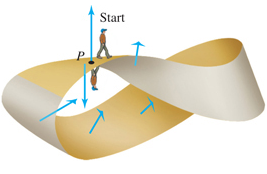
\includegraphics[scale=1]{Mobius}
\end{center}

% % % % %
\end{enumerate}
\end{document}